\documentclass[aspectratio=169,11pt]{beamer}
\usetheme{Madrid}
\usecolortheme{default}
\setbeamertemplate{navigation symbols}{}
\setbeamertemplate{footline}[frame number]
\setbeamertemplate{itemize items}[circle]
\usepackage[T1]{fontenc}
\usepackage[utf8]{inputenc}
\usepackage{lmodern}
\usepackage{graphicx}
\usepackage{xcolor}
\graphicspath{{plots/}}

\definecolor{accent}{RGB}{25,72,140}
\definecolor{muted}{RGB}{85,85,85}

\setbeamercolor{title}{fg=accent}
\setbeamercolor{frametitle}{fg=accent}
\setbeamercolor{structure}{fg=accent}
\setbeamercolor{normal text}{fg=black,bg=white}

\title{Strategic Allocation Framework}
\subtitle{Data, Horizon, Macro Inputs, and Benchmark Behavior}
\author{XOPTPOE}
\date{}

\begin{document}

\begin{frame}
  \titlepage
\end{frame}

\begin{frame}{Investment Universe and Horizon}
\begin{columns}[T,totalwidth=\textwidth]
\column{0.54\textwidth}
\textbf{9 asset classes}
\begin{itemize}
  \item US Equities
  \item Euro Area Equities
  \item Japan Equities
  \item China Equities
  \item Emerging Market Equities
  \item US Treasuries 7--10Y
  \item Investment Grade Credit
  \item Gold
  \item US REITs
\end{itemize}

\column{0.46\textwidth}
\textbf{Time horizon}
\begin{itemize}
  \item Main strategic horizon: 5 years
  \item Secondary reference horizon: 10 years
  \item Main benchmark used in the deck: robust 5-year portfolio benchmark
  \item Strategic asset allocation, not short-term tactical trading
\end{itemize}
\end{columns}
\end{frame}

\begin{frame}{What Data the Model Uses}
\textbf{Macro-financial state variables}
\begin{itemize}
  \item \texttt{infl\_US}, \texttt{unemp\_US}, \texttt{short\_rate\_US}, \texttt{long\_rate\_US}
  \item \texttt{infl\_EA}, \texttt{unemp\_EA}, \texttt{short\_rate\_EA}, \texttt{long\_rate\_EA}
  \item \texttt{infl\_JP}, \texttt{unemp\_JP}, \texttt{short\_rate\_JP}, \texttt{long\_rate\_JP}
  \item \texttt{usd\_broad}, \texttt{vix}, \texttt{us\_real10y}, \texttt{ig\_oas}, \texttt{oil\_wti}
\end{itemize}
\vspace{0.6em}
\textbf{Regional coverage}
\begin{itemize}
  \item United States
  \item Euro Area
  \item Japan
\end{itemize}
\vspace{0.5em}
{\small\color{muted}These variables define the scenario state used to generate long-horizon return views and portfolio allocations across the 9 sleeves.}
\end{frame}

\begin{frame}{Model Logic}
\begin{itemize}
  \item Step 1: form long-horizon sleeve-level return views
  \item Step 2: map those views into a full 9-sleeve allocation
  \item Step 3: evaluate the benchmark through return, concentration, and portfolio structure
\end{itemize}
\vspace{0.8em}
\textbf{Practical interpretation}
\begin{itemize}
  \item the model matters only if both the prediction layer and the portfolio layer are interpretable
  \item the next slides show that benchmark behavior is coherent at both levels
\end{itemize}
\end{frame}

\begin{frame}{Benchmark Overview}
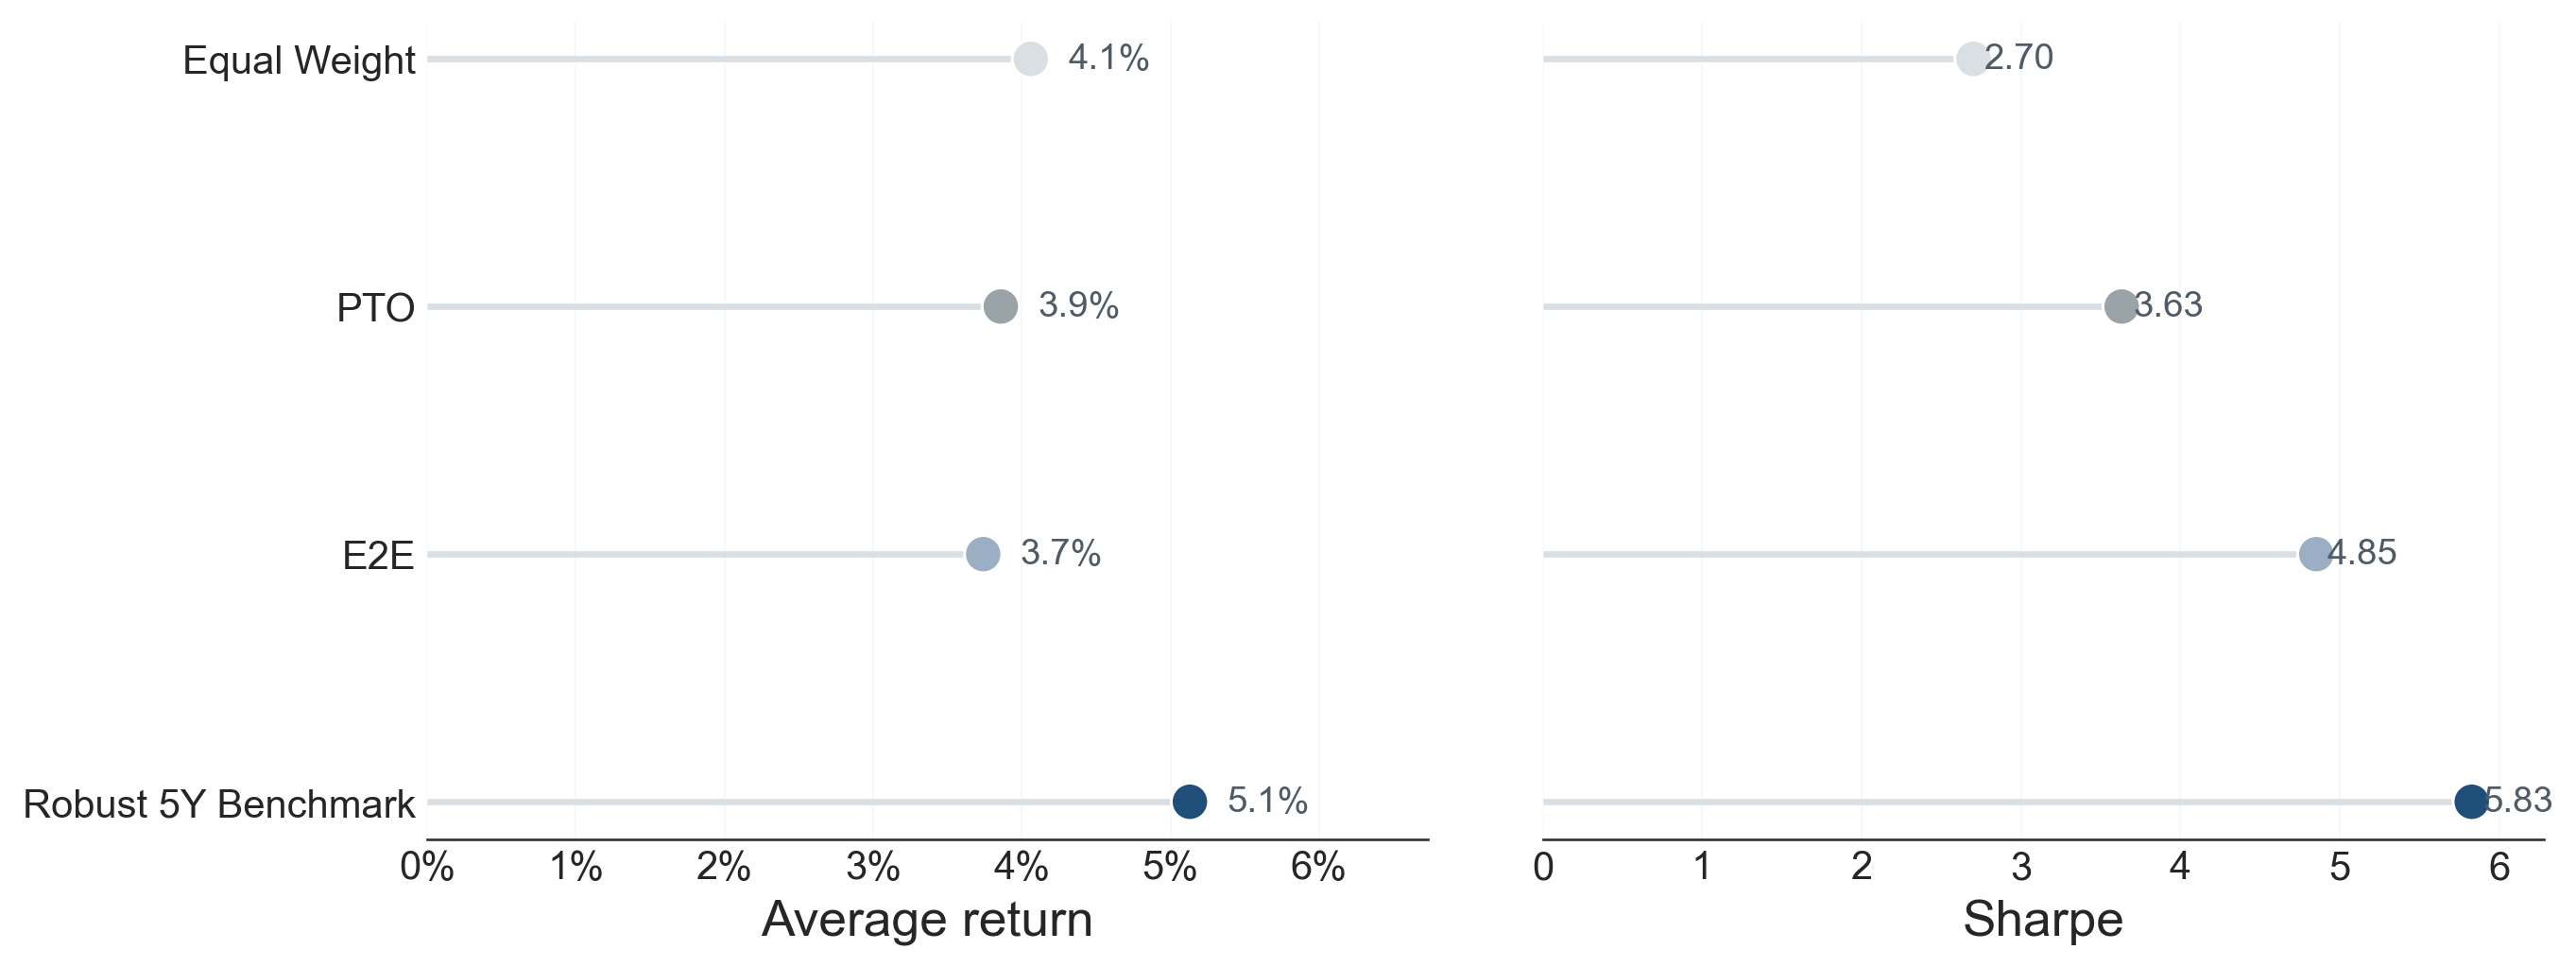
\includegraphics[width=\linewidth,height=0.82\textheight,keepaspectratio]{benchmark_60_overview.pdf}
\end{frame}

\begin{frame}{Prediction Quality}
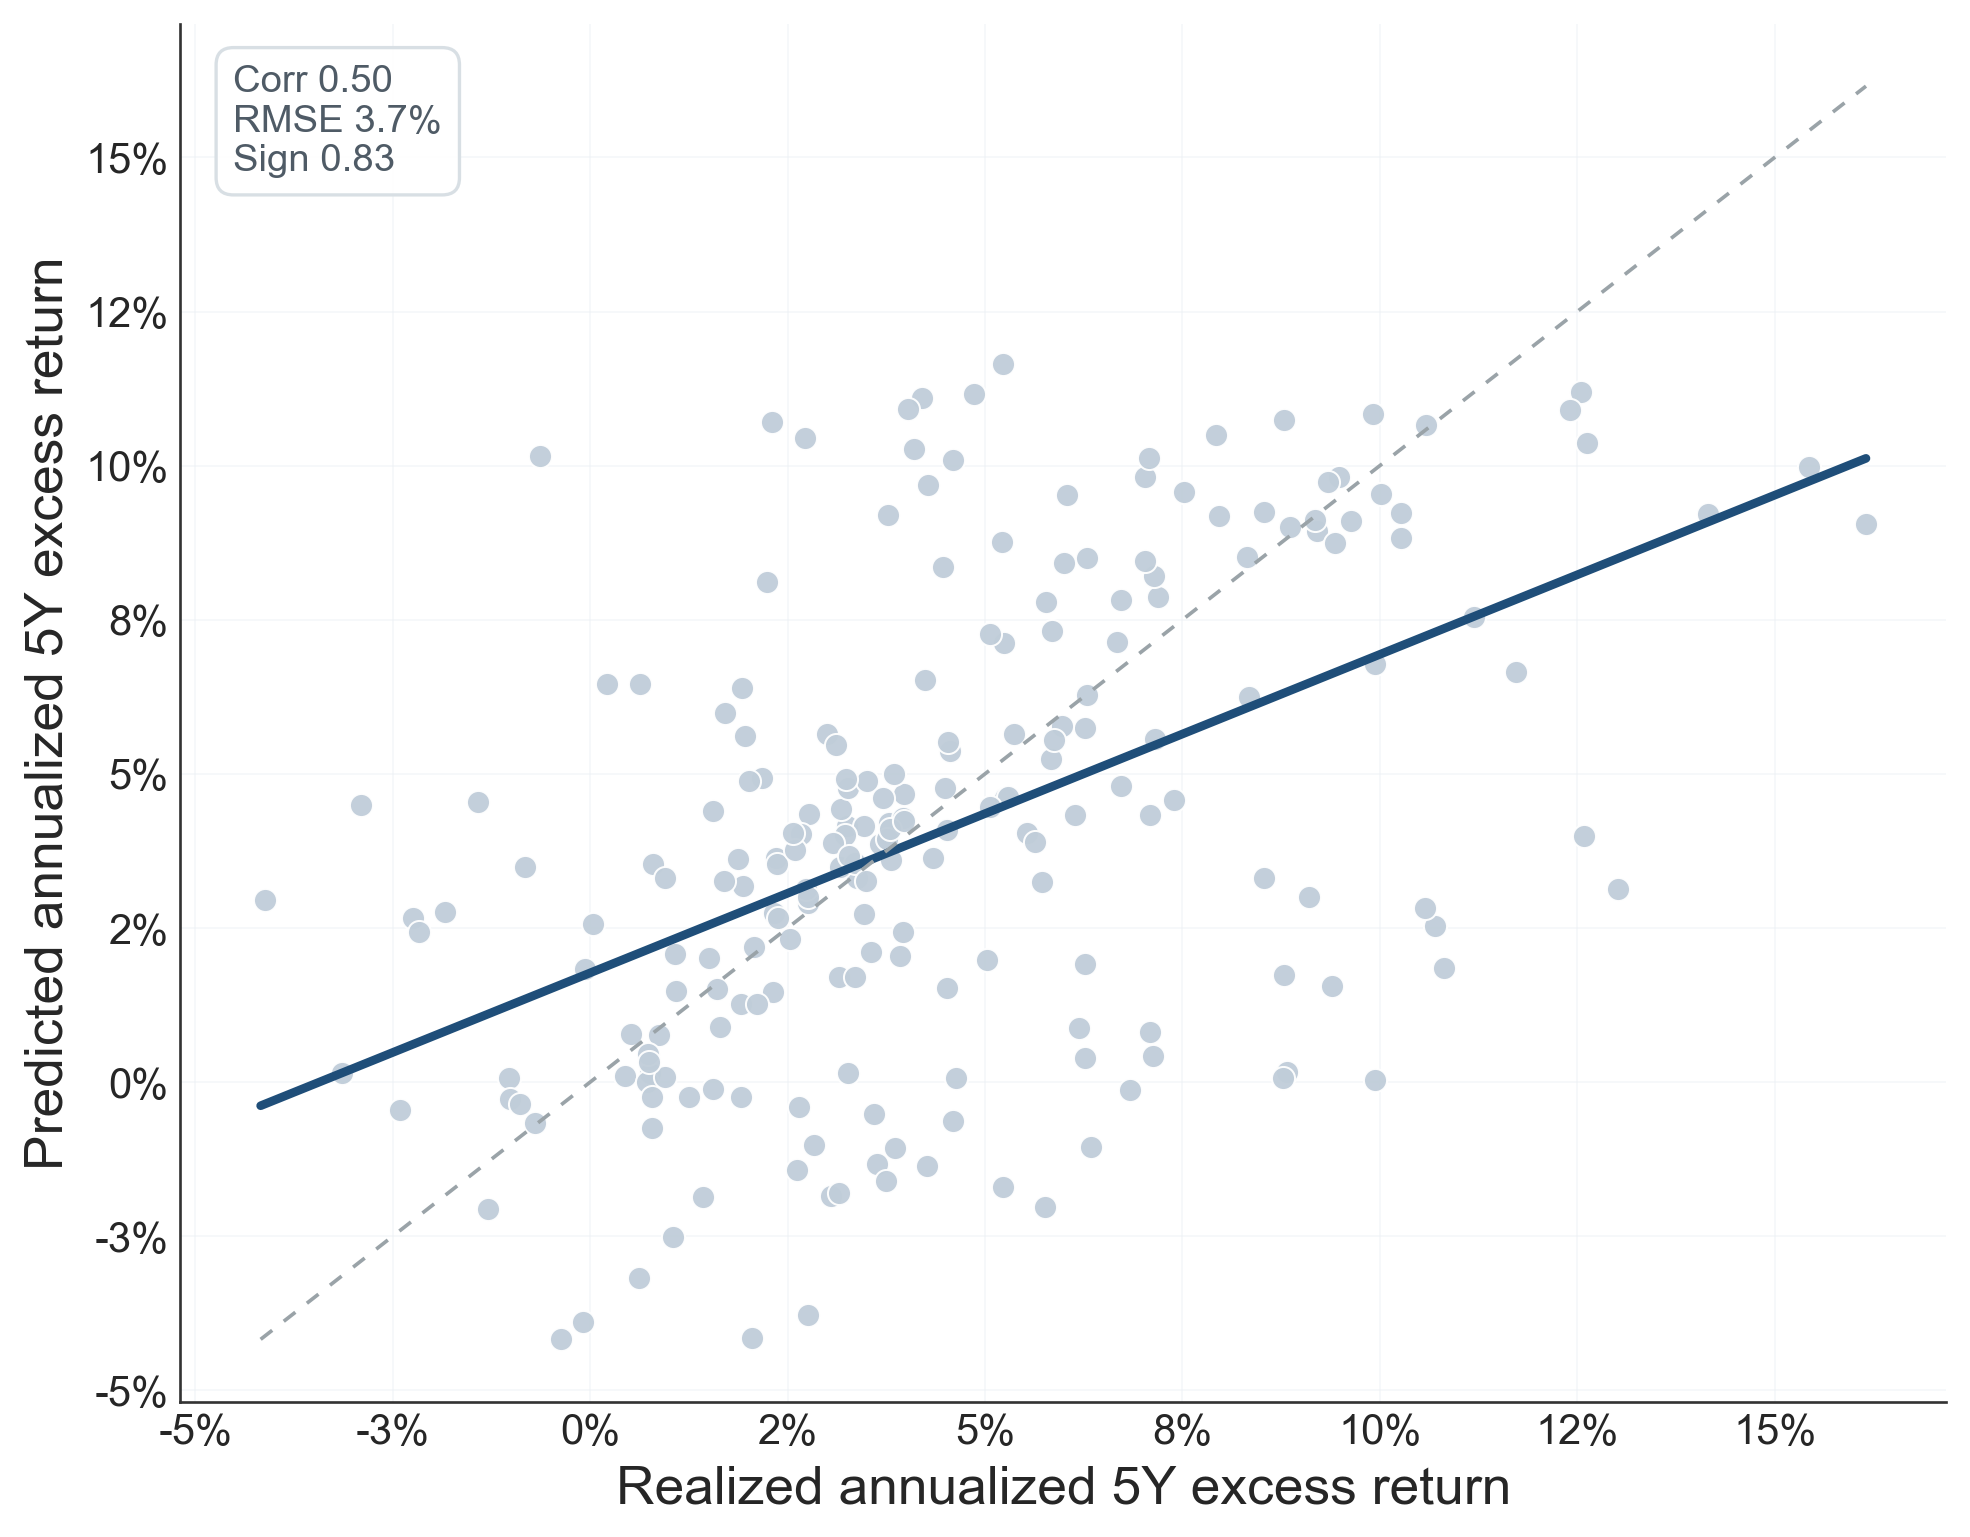
\includegraphics[width=\linewidth,height=0.82\textheight,keepaspectratio]{prediction_scatter_60.pdf}
\end{frame}

\begin{frame}{Recent 5Y Return Views}
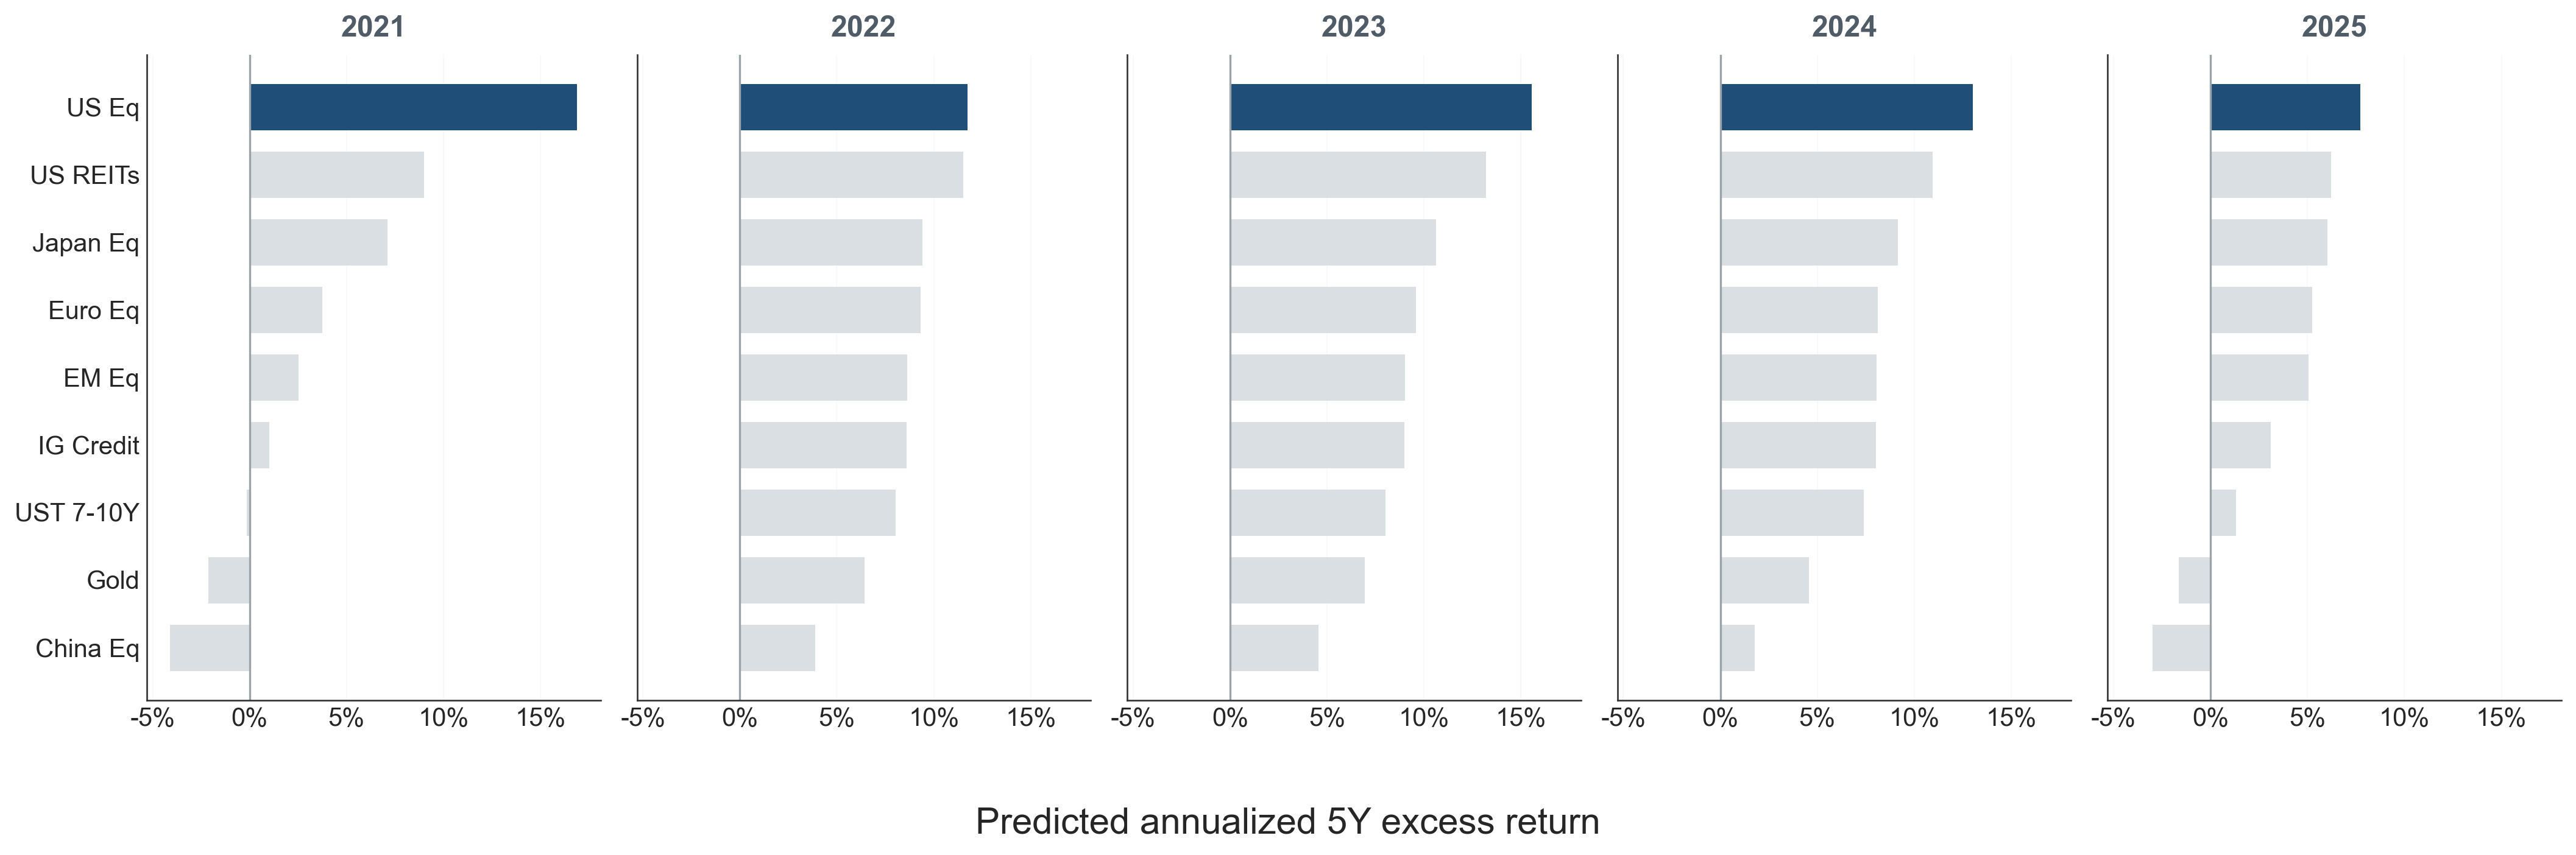
\includegraphics[width=\linewidth,height=0.82\textheight,keepaspectratio]{recent_prediction_snapshot_5y.pdf}
\end{frame}

\begin{frame}{Recent 5Y Portfolio Allocations}
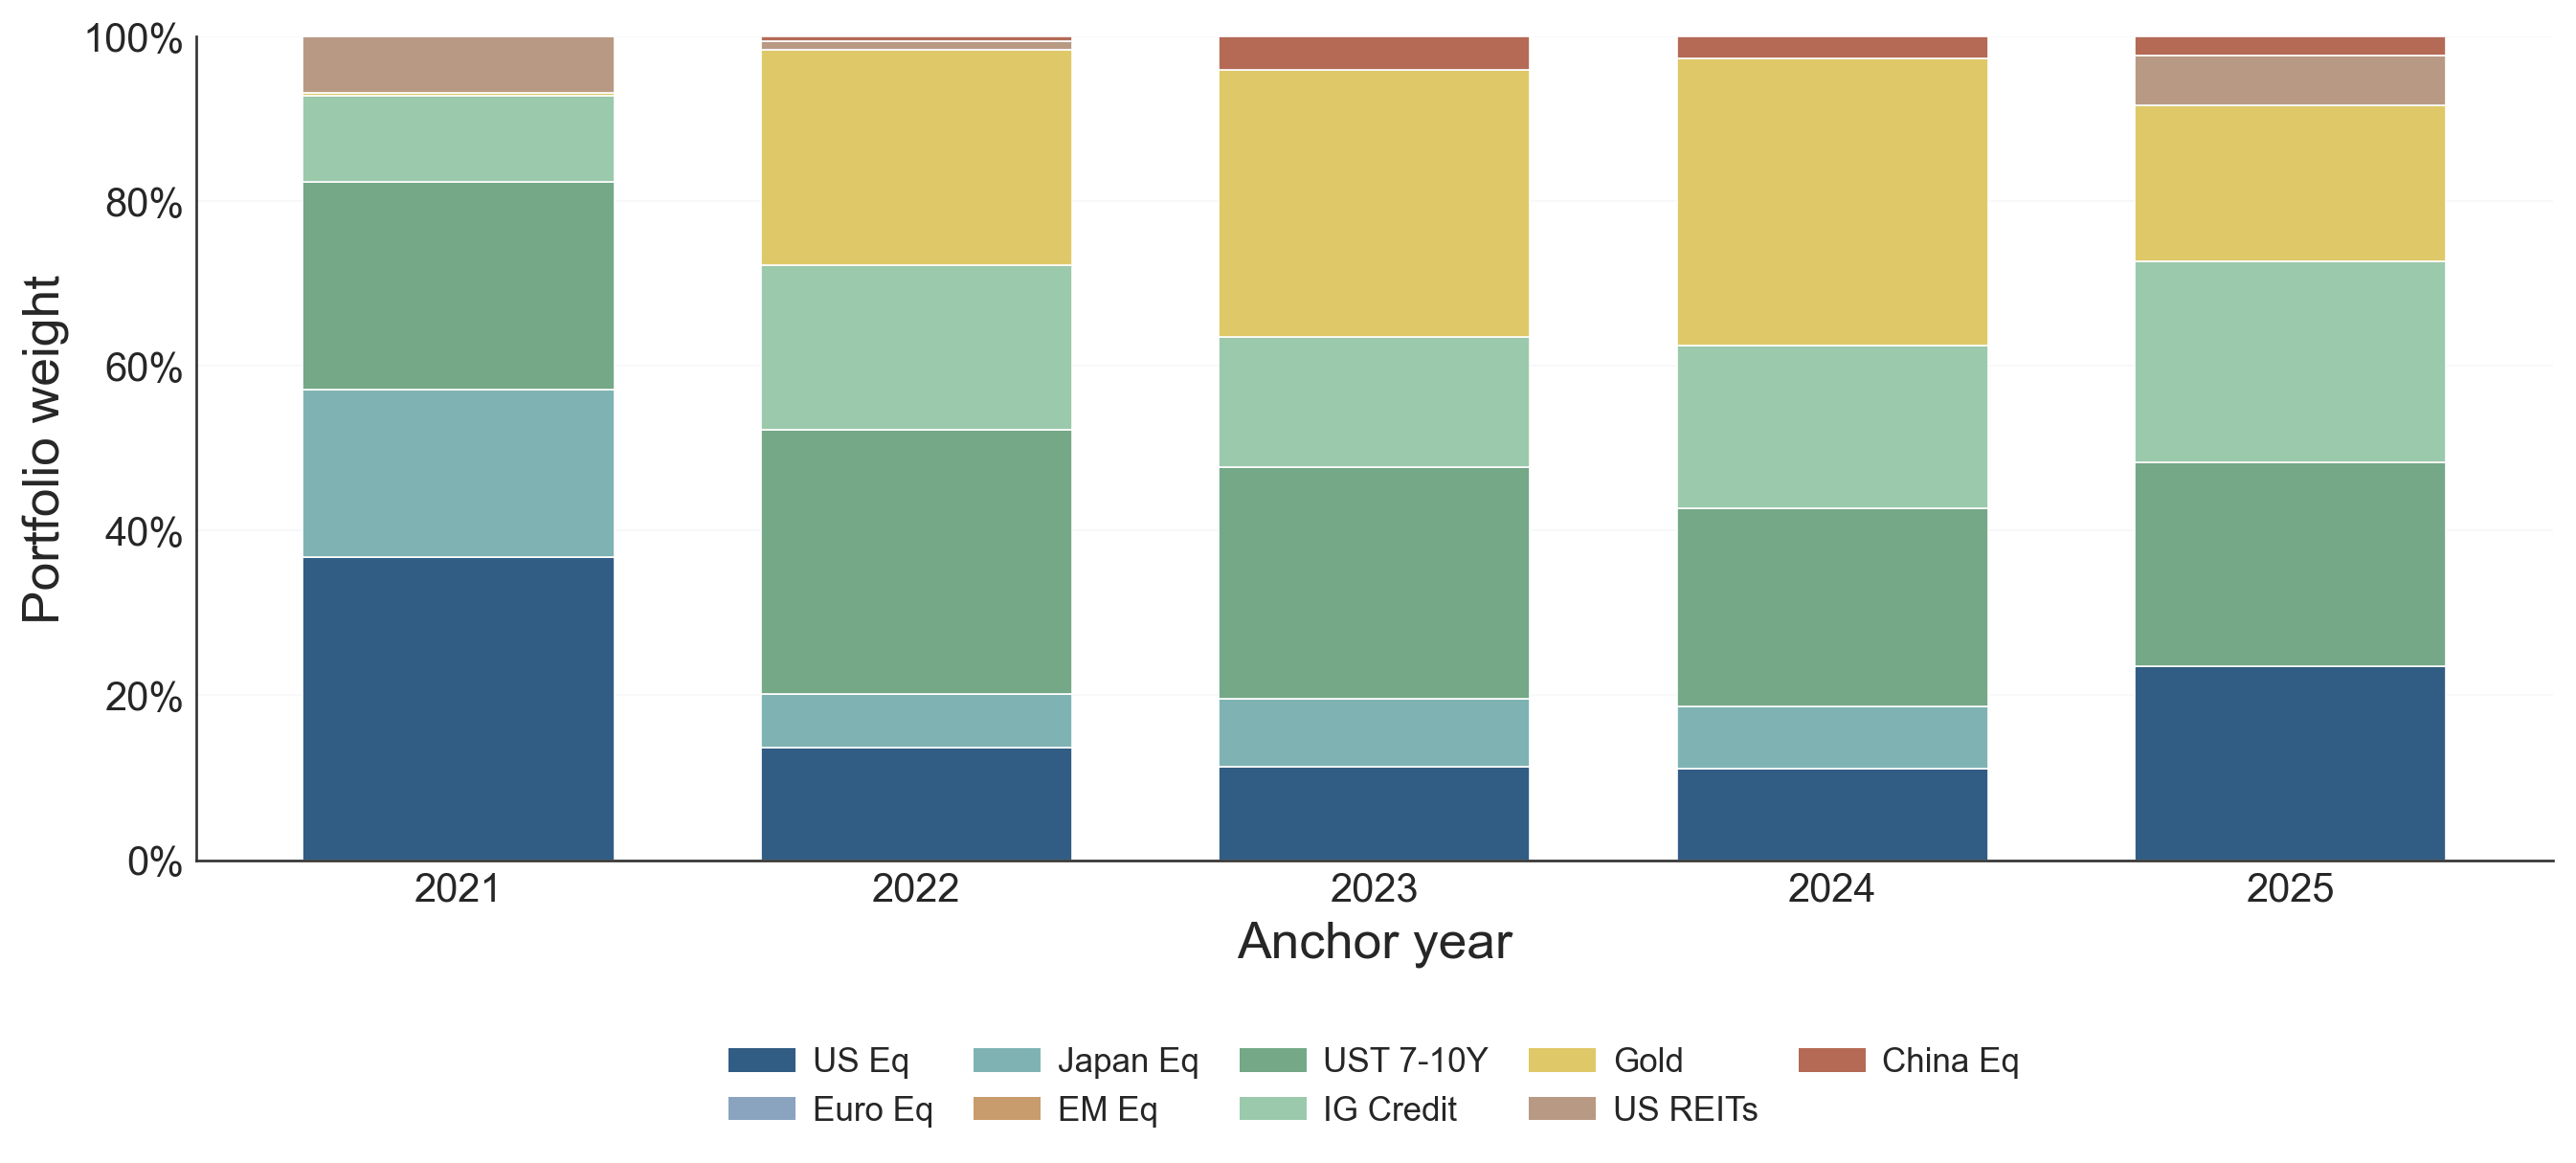
\includegraphics[width=\linewidth,height=0.82\textheight,keepaspectratio]{recent_portfolio_snapshot_5y.pdf}
\end{frame}

\begin{frame}{Walk-Forward Portfolio Path}
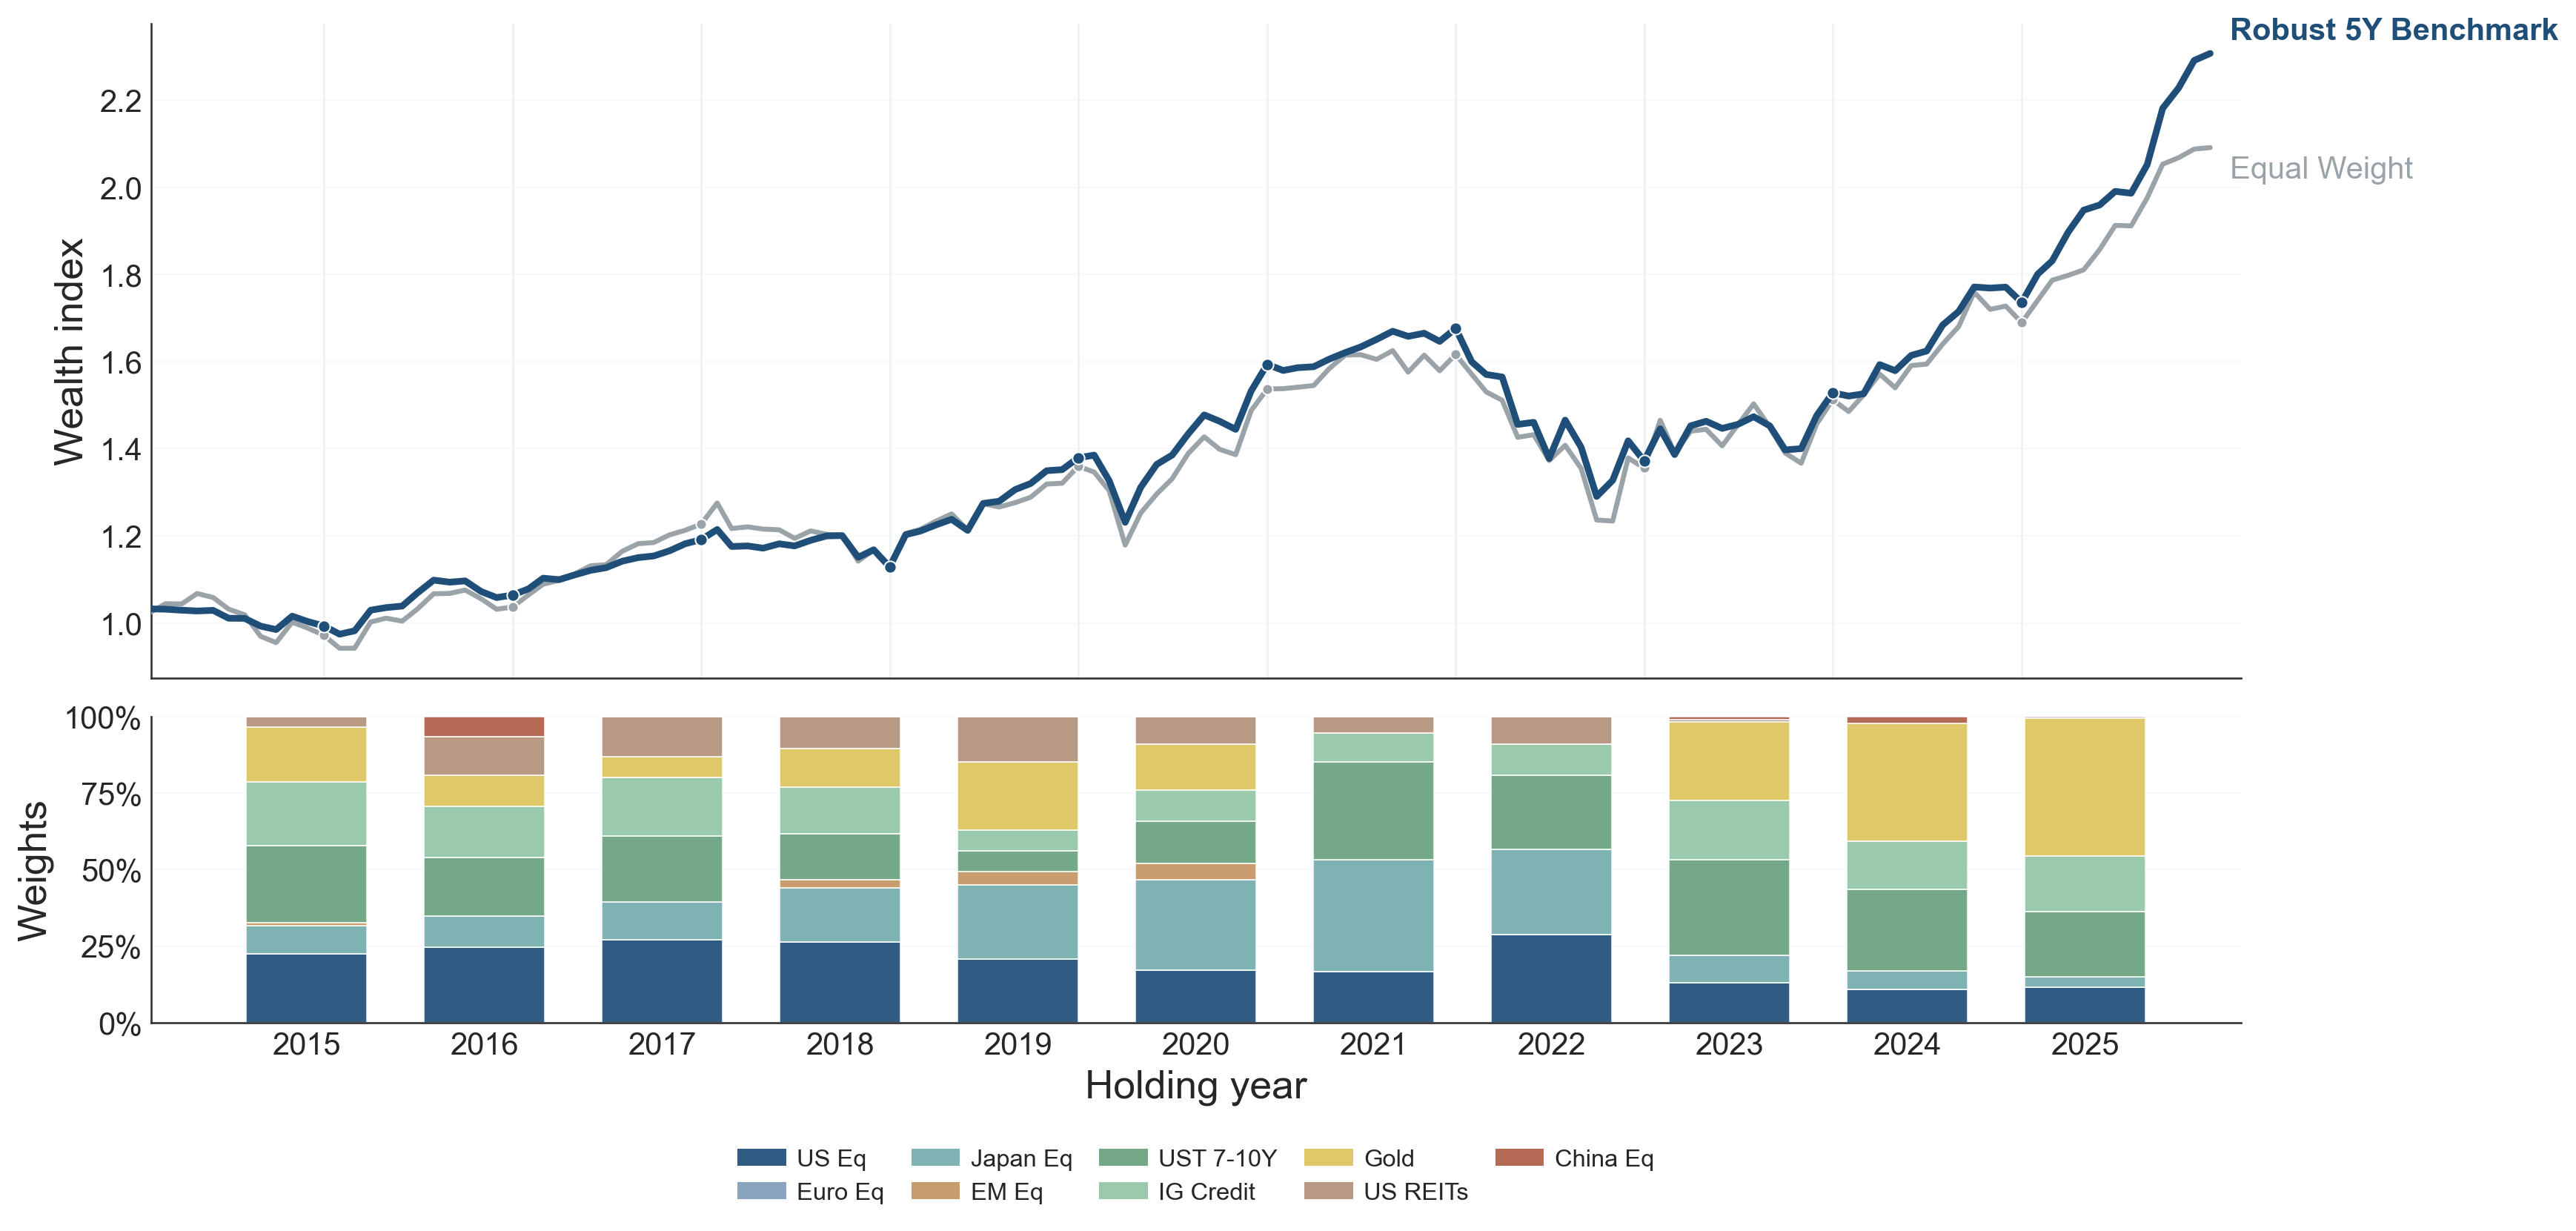
\includegraphics[width=\linewidth,height=0.82\textheight,keepaspectratio]{portfolio_wealth_path_best_60.pdf}
\end{frame}

\begin{frame}{Portfolio Allocation Structure}
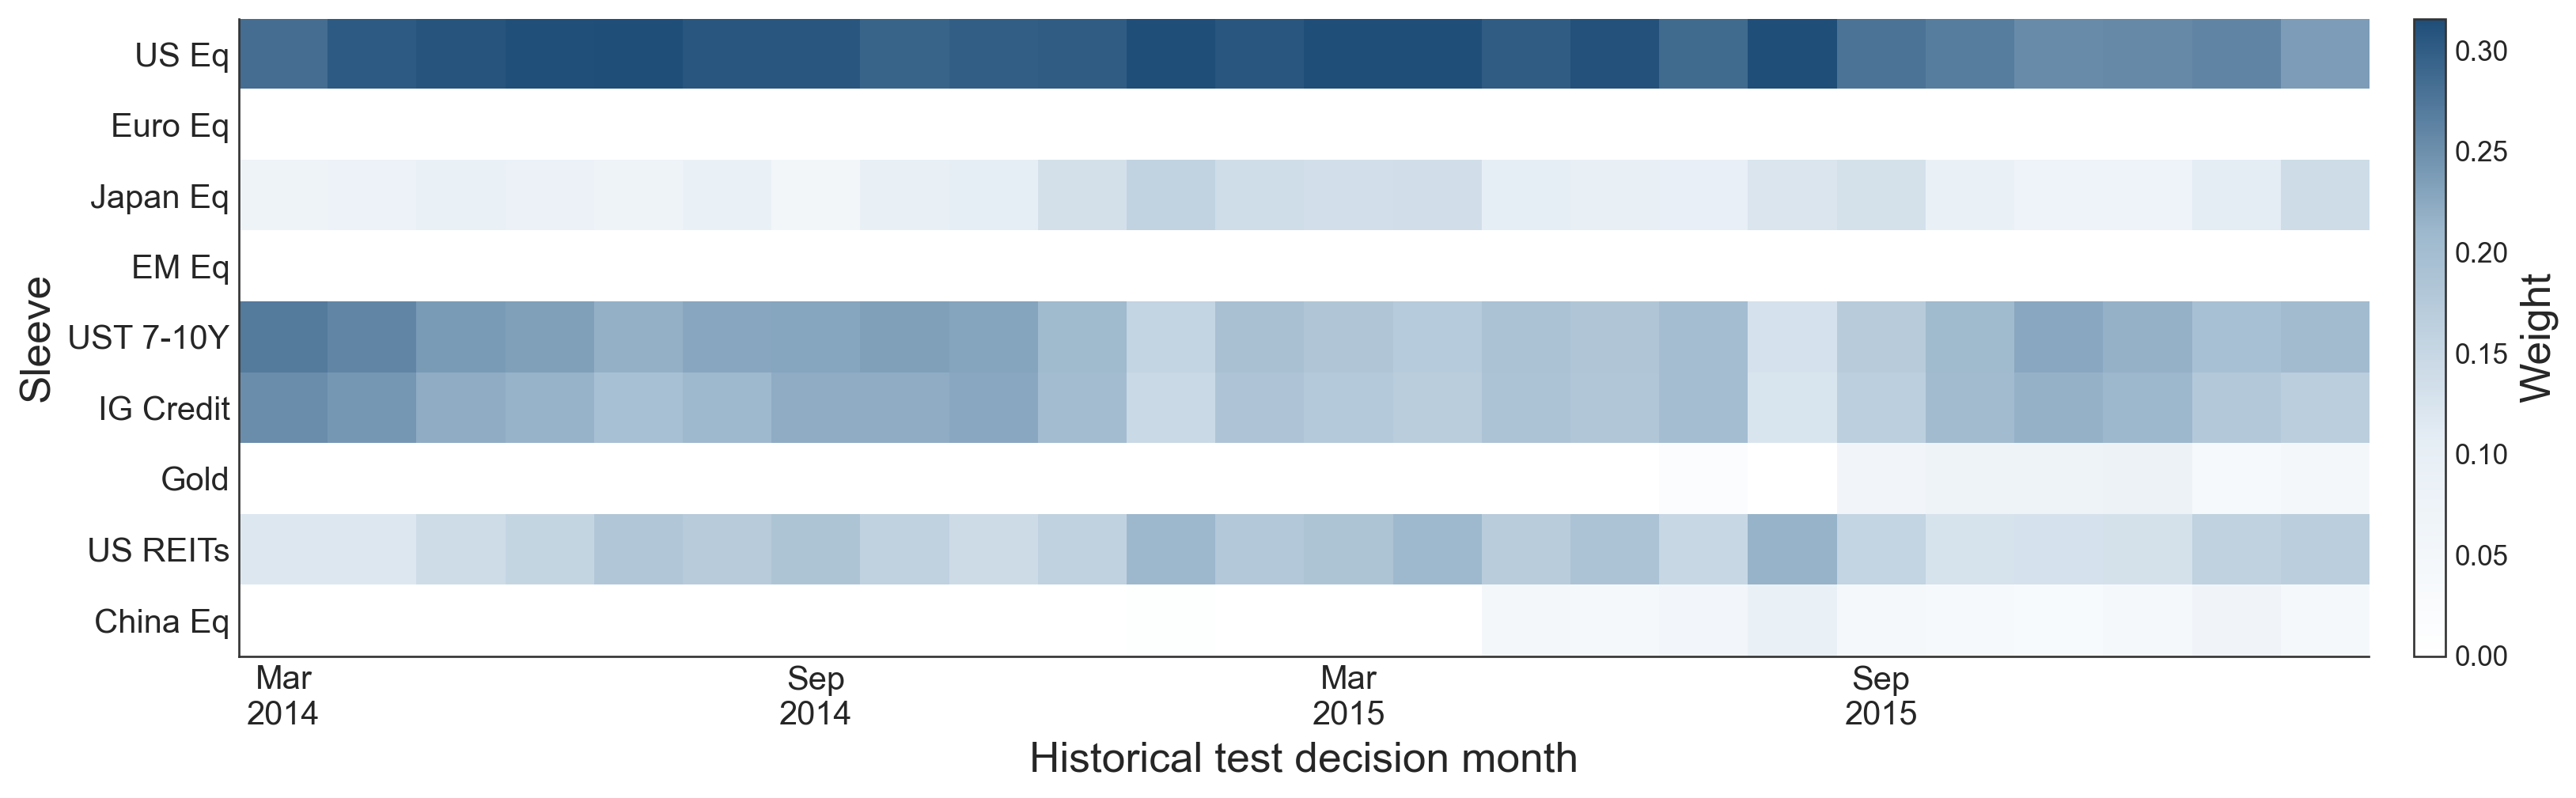
\includegraphics[width=\linewidth,height=0.82\textheight,keepaspectratio]{allocation_heatmap_best_60.pdf}
\end{frame}

\end{document}
